% ============================================================================
% UNIDADE IV: CAPÍTULO 15: SEMINÁRIO FINAL DE INTEGRAÇÃO (AV3, 50%)
% ============================================================================

\aberturaModulo{UNIDADE IV}{SÍNTESE TERRITORIAL E SEMINÁRIO INTEGRADOR}{Encontro 15 $\bullet$ Projeto Final Aplicado e Defesa Oral: AV3 (50\%)}{%
Esta unidade conclusiva promove a síntese epistemológica, estratégica e econômico-financeira de todo o percurso formativo da disciplina. O foco recai sobre a estruturação, a defesa oral e a avaliação do \textbf{Projeto Final Integrador (AV3, 50\% da nota)}, conectando a leitura territorial crítica da Unidade I (APLs, SRIs, Hélice Quádrupla/Quíntupla e Tecnologia Social), a modelagem de oportunidade e estratégia da Unidade II (TAM/SAM/SOM, Canvas, PI e fomento regional) e a engenharia de viabilidade da Unidade III (Matriz Locacional, VPL, TIR, \textit{Valuation} e retenção de valor). Ao final, orienta-se a conversão do projeto técnico em artigo científico para fóruns de Planejamento Urbano e Regional e Gestão (ANPUR, ENANPAD e ENGEMA).%
}

\chapter{Seminário Final de Integração: Ecossistemas, Negócios e Viabilidade Territorial}
\tagAV{AV3 (50\%)}\ \tagTerritorio

\begin{capObjetivos}
Ao concluir este capítulo, você será capaz de:
\begin{itemize}[leftmargin=1.4em, itemsep=2pt]
  \item Articular, em um único projeto aplicado, o diagnóstico territorial (Unidade I), a modelagem estratégica do negócio ou política de inovação (Unidade II) e a viabilidade locacional e econômico-financeira (Unidade III);
  \item Aplicar integralmente a \textbf{Matriz Oficial da Rubrica AV3} (30\% Leitura Territorial, 30\% Estratégia e Modelo, 25\% Viabilidade e \textit{Valuation}, 15\% Comunicação e Defesa) para auditar a qualidade do próprio trabalho;
  \item Estruturar uma defesa oral objetiva em \textbf{10 slides (20 minutos de apresentação + 10 minutos de arguição)}, equilibrando rigor conceitual e evidência quantitativa;
  \item Traduzir o relatório técnico do Projeto Final Integrador em manuscrito científico apto à submissão em eventos e periódicos de Planejamento Urbano e Regional e Gestão (ANPUR, ENANPAD, ENGEMA).
\end{itemize}
\end{capObjetivos}

\begin{capRevisao}
Antes de montar a versão definitiva do Projeto Final Integrador (AV3), certifique-se de dominar os seguintes pilares das unidades anteriores:
\begin{itemize}[leftmargin=1.4em, itemsep=2pt]
  \item \textbf{Unidade I (Território e Ecossistemas):} superação do isomorfismo institucional; cálculo de concentração de mercado ($\text{HHI}$); distinção entre APLs, Sistemas Regionais de Inovação (SRIs) e Hélice Quádrupla/Quíntupla; Teoria da Mudança e Tecnologia Social.
  \item \textbf{Unidade II (Processo e Estratégia):} lógica \textit{Effectuation} vs.\ \textit{Causation}; funil $\text{TAM/SAM/SOM}$; métricas de tração ($\text{LTV/CAC}$, \textit{Burn Rate} e \textit{Runway}); proteção de Propriedade Intelectual (PI) e instrumentos regionais de fomento (FINEP, BNDES, BNB, FAPESB).
  \item \textbf{Unidade III (Projetos e Viabilidade):} Matriz Locacional Ponderada ($S_j$); Fluxo de Caixa Livre ($\text{FCL}$); $\text{VPL}$, $\text{TIR}$, $\text{MTIR}$, $\text{VAUE}$ e \textit{Payback} Descontado; $\text{WACC}$, Valor Terminal de Gordon, \textit{Enterprise Value} ($\text{EV}$), \textit{Equity Value} ($EqV$) e Método de \textit{Venture Capital}.
\end{itemize}
\end{capRevisao}

\etapa{3}{Articulação Epistemológica, Rubrica AV3 e Roteiro de Defesa}

\begin{boxSimbolo}[Vocabulário Conceitual e Símbolos do Capítulo]
Na avaliação conclusiva da disciplina, $N_{\text{AV3}}$ representa a nota ponderada obtida no Projeto Final Integrador (em escala de $0{,}0$ a $10{,}0$), composta por quatro dimensões: $L_T$, que mede a \textbf{Leitura Territorial e Ecossistêmica} (peso $30\%$); $E_M$, referente a \textbf{Estratégia, Oportunidade e Modelo de Negócio} (peso $30\%$); $V_F$, correspondente a \textbf{Viabilidade Locacional, Financeira e \textit{Valuation}} (peso $25\%$); e $C_D$, que avalia \textbf{Comunicação Técnica e Defesa Oral} (peso $15\%$). A Média Final da disciplina ($M_F$) integra as três avaliações pela ponderação $\text{AV1} \cdot 0{,}30 + \text{AV2} \cdot 0{,}20 + \text{AV3} \cdot 0{,}50$. Complementarmente, $\text{IRV}$ designa o Índice de Retenção Territorial de Valor (proporção dos gastos operacionais, massa salarial e excedentes que permanece no território de origem), e $\text{TRL}$ indica o \textit{Technology Readiness Level} (nível de maturidade tecnológica, de $1$ a $9$).
\end{boxSimbolo}

\subsection{Articulação Epistemológica entre as Unidades I, II e III}

Um projeto de empreendedorismo tecnológico voltado ao desenvolvimento territorial fracassa quando trata o território como mero suporte físico neutro ou quando adota modelos importados sem aderência produtiva. A arquitetura desta disciplina exige uma tripla amarração lógica que integra diagnóstico, estratégia e engenharia financeira.

Na \textbf{Ancoragem Territorial (Unidade I)}, o projeto parte da leitura crítica das vocações, dos gargalos e das assimetrias do território. Superando o isomorfismo de parques tecnológicos descontextualizados, você identifica como o empreendimento se acopla a Arranjos Produtivos Locais (APLs), fortalece a eficiência coletiva, mobiliza a Hélice Quádrupla/Quíntupla e evita o aprisionamento cognitivo (\textit{lock-in}). Quando há foco socioambiental, o projeto explicita a Teoria da Mudança e os mecanismos contra o desvio de missão (\textit{mission drift}).

Na \textbf{Arquitetura Estratégica e de Mercado (Unidade II)}, com o problema territorial delimitado, a proposta converte a dor identificada em oportunidade tecnológica ou de impacto. O funil $\text{TAM/SAM/SOM}$ quantifica a demanda real alcançável, o \textit{Business Model Canvas} (ou \textit{Lean Canvas}) alinha proposta de valor, canais e estrutura de custos, o plano de PI protege ativos críticos (patentes, marcas, Indicações Geográficas ou licenças abertas de Tecnologia Social) e a estratégia de capital combina receitas próprias com editais de fomento regional (FAPESB, BNB/ETENE, FINEP e BNDES).

No \textbf{Rigor Locacional, Viabilidade e Retenção de Valor (Unidade III)}, a estratégia fecha a conta sem sacrificar o território. A decisão locacional apoia-se em matriz multicritério ponderada, os investimentos ($\text{CAPEX}$) e despesas ($\text{OPEX}$) alimentam um Fluxo de Caixa Livre ($\text{FCL}$) descontado pela $\text{TMA}$ ou pelo $\text{WACC}$, e indicadores como $\text{VPL}$, $\text{TIR}$, $\text{MTIR}$ e \textit{Payback} Descontado atestam a sustentabilidade econômica. Nesse estágio, o \textit{Valuation} (FCD ou Método VC) dialoga com o Índice de Retenção Territorial de Valor ($\text{IRV}$), indicando que parcela expressiva da riqueza gerada irriga fornecedores, trabalho qualificado e cadeias locais.

\subsection{Matriz Oficial da Rubrica AV3 (50\% da Nota)}

O Seminário Final Integrador é composto pela entrega do relatório técnico-estratégico e pela \textbf{defesa oral presencial de 20 minutos de apresentação seguidos de 10 minutos de arguição} pela banca. A nota $N_{\text{AV3}}$ obedece à ponderação oficial formalizada no modelo matemático abaixo.

\begin{boxFormula}[Modelo Matemático da Rubrica Oficial AV3 e Média Final]
A nota do Projeto Final Integrador ($N_{\text{AV3}}$) é a média ponderada dos quatro blocos avaliativos, cada qual pontuado de $0{,}0$ a $10{,}0$:
\[
N_{\text{AV3}} = 0{,}30\,L_T + 0{,}30\,E_M + 0{,}25\,V_F + 0{,}15\,C_D
\]
A Média Final ($M_F$) na disciplina integra as três avaliações oficiais:
\[
M_F = 0{,}30\,\text{AV1} + 0{,}20\,\text{AV2} + 0{,}50\,N_{\text{AV3}}
\]
Como indicador complementar de enraizamento econômico, define-se o Índice de Retenção Territorial de Valor ($\text{IRV}$):
\[
\text{IRV} = \frac{\text{Gastos com Fornecedores Locais} + \text{Massa Salarial Local} + \text{Reinvestimento Territorial}}{\text{Valor Total Gerado / Desembolso Operacional Total}}
\]
\end{boxFormula}

A Figura~\ref{fig:fig15_av3} ilustra essa ponderação oficial da Rubrica AV3 e o tripé de integração entre território, modelo de negócio e viabilidade econômico-financeira.

\begin{figure}[H]
  \centering
  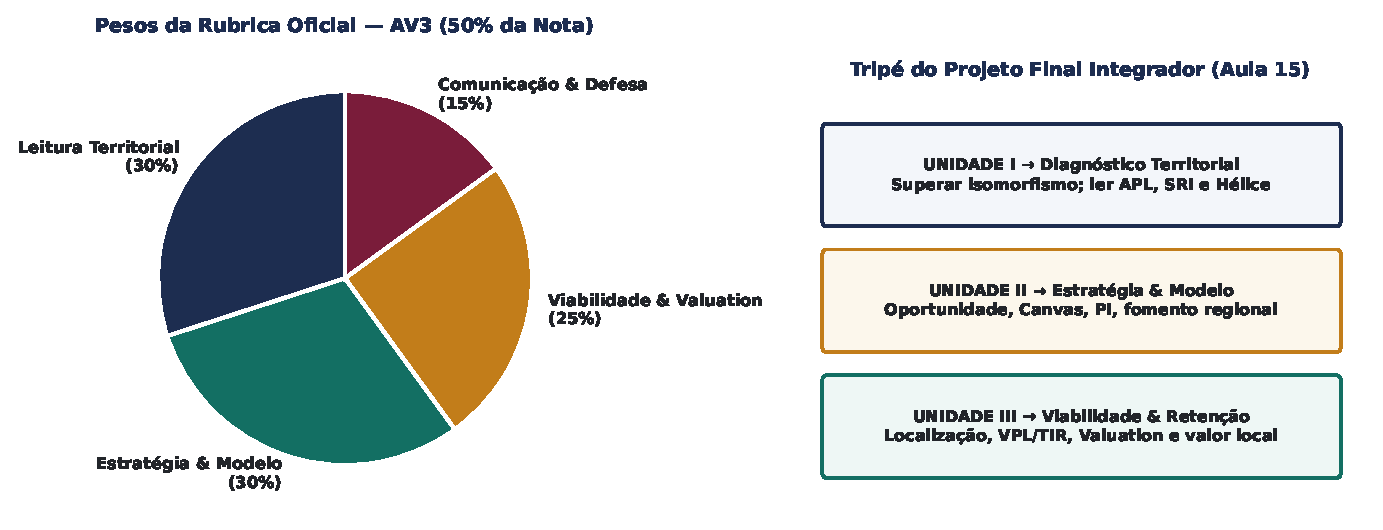
\includegraphics[width=0.94\textwidth]{figures/fig15_projeto_final_av3.pdf}
  \caption{Pesos oficiais da Rubrica AV3 (50\% da nota) e tripé de integração entre território, modelo de negócio e viabilidade econômico-financeira.}
  \label{fig:fig15_av3}
\end{figure}

A Tabela~\ref{tab:rubrica_av3} detalha os níveis de desempenho esperados em cada dimensão da rubrica oficial.

\begin{table}[H]
\centering
\caption{Matriz Oficial de Avaliação do Projeto Final Integrador (AV3).}
\label{tab:rubrica_av3}
\renewcommand{\arraystretch}{1.22}
\footnotesize
\begin{tabularx}{\textwidth}{@{}p{2.7cm} c >{\raggedright\arraybackslash}X >{\raggedright\arraybackslash}X@{}}
  \toprule
  \rowcolor{etIndigo}
  \textcolor{white}{\bfseries Dimensão} & \textcolor{white}{\bfseries Peso} & \textcolor{white}{\bfseries Padrão Insuficiente / Regular ($0{,}0$–$6{,}9$)} & \textcolor{white}{\bfseries Padrão Bom / Excelente ($7{,}0$–$10{,}0$)} \\
  \midrule
  \textbf{1. Leitura Territorial e Ecossistêmica ($L_T$)} & \textbf{30\%} & Descrição genérica da região; importação acrítica de modelos externos (isomorfismo); ausência de dados de APL, SRI ou atores da Hélice. & Diagnóstico territorial com dados empíricos; articulação precisa com APL/SRI, Hélice Quádrupla/Quíntupla, proximidades de Boschma e impacto socioambiental. \\
  \rowcolor{bgGray}
  \textbf{2. Estratégia, Oportunidade e Modelo ($E_M$)} & \textbf{30\%} & Oportunidade vaga sem TAM/SAM/SOM; Canvas desconectado do problema; omissão de PI e de fontes reais de fomento regional. & Funil TAM/SAM/SOM auditável; Canvas coerente com métricas (LTV/CAC, Burn/Runway); estratégia clara de PI e captação (FINEP, BNDES, BNB, FAPESB). \\
  \textbf{3. Viabilidade e \textit{Valuation} ($V_F$)} & \textbf{25\%} & Escolha locacional intuitiva; fluxo de caixa com premissas sem lastro; ausência de TMA/WACC, VPL, TIR ou confusão entre EV e Equity. & Matriz locacional ponderada; FCL consistente com CAPEX/OPEX; cálculo correto de VPL, TIR, Payback, WACC, \textit{Valuation} (FCD/VC) e análise de sensibilidade/IRV. \\
  \rowcolor{bgGray}
  \textbf{4. Comunicação e Defesa Oral ($C_D$)} & \textbf{15\%} & Slides poluídos, extrapolação severa dos 20 min, leitura integral de texto e respostas defensivas ou imprecisas na arguição. & Síntese visual limpa em 10 slides dentro dos 20 min; domínio conceitual e numérico na arguição de 10 min, reconhecendo limites e premissas. \\
  \bottomrule
\end{tabularx}
\end{table}

\subsection{Roteiro Estruturado de Apresentação em 10 Slides (20 min + 10 min)}

Para cumprir rigorosamente o tempo de 20 minutos, recomenda-se a cadência média de 2 minutos por slide, reservando 10 minutos finais para a arguição técnica da banca:

\begin{table}[H]
\centering
\caption{Roteiro padrão de 10 slides para a Defesa Oral da AV3 (20 minutos).}
\label{tab:roteiro_10_slides}
\renewcommand{\arraystretch}{1.18}
\footnotesize
\begin{tabularx}{\textwidth}{@{}c p{4.0cm} c >{\raggedright\arraybackslash}X@{}}
  \toprule
  \rowcolor{etTeal}
  \textcolor{white}{\bfseries Slide} & \textcolor{white}{\bfseries Título Funcional} & \textcolor{white}{\bfseries Tempo} & \textcolor{white}{\bfseries Conteúdo Essencial e Evidências Exigidas} \\
  \midrule
  \textbf{1} & Título, Equipe e Recorte Territorial & 1 min & Nome do projeto/empreendimento, território-alvo (município/região), problema central e vínculo com APL/SRI. \\
  \rowcolor{bgGray}
  \textbf{2} & Diagnóstico Territorial e Ecossistêmico & 2 min & Dados do território, estrutura de mercado ($\text{HHI}$ ou densidade produtiva), gargalos e atores da Hélice Quádrupla/Quíntupla. \\
  \textbf{3} & Oportunidade e Enquadramento Tecnológico & 2 min & Origem da oportunidade (\textit{discovery}/\textit{creation}), maturidade tecnológica ($\text{TRL}$), solução proposta e diferencial frente a incumbentes. \\
  \rowcolor{bgGray}
  \textbf{4} & Mercado (\text{TAM/SAM/SOM}) e Impacto & 2 min & Funil quantificado de mercado alcançável e, quando aplicável, Teoria da Mudança (insumos, produtos, resultados, impacto). \\
  \textbf{5} & Modelo de Negócio e Tração & 2 min & Síntese do \textit{Canvas} (proposta de valor, segmentos, receitas/custos) e métricas unitárias ($\text{CAC}$, $\text{LTV}$, $\text{LTV/CAC}$). \\
  \rowcolor{bgGray}
  \textbf{6} & Propriedade Intelectual e Fomento & 2 min & Estratégia de PI (patente, registro, IG, Tecnologia Social) e escada de capital (subvenção FAPESB/FINEP, crédito BNB/BNDES). \\
  \textbf{7} & Decisão Locacional Multicritério & 2 min & Tabela resumida da Matriz Locacional comparando alternativas municipais/distritais e justificando os pesos adotados. \\
  \rowcolor{bgGray}
  \textbf{8} & Viabilidade Econômico-Financeira & 3 min & $\text{CAPEX}$, $\text{OPEX}$, $\text{FCL}$ projetado, $\text{TMA}/\text{WACC}$, $\text{VPL}$, $\text{TIR}$/\text{MTIR}, \textit{Payback} Descontado e análise de sensibilidade. \\
  \textbf{9} & \textit{Valuation} e Retenção Territorial & 2 min & Estimativa de $\text{EV}$ e \textit{Equity Value} (FCD ou VC), diluição (se houver rodada) e cálculo do $\text{IRV}$ / externalidades locais. \\
  \rowcolor{bgGray}
  \textbf{10} & Riscos, Cronograma e Encaminhamentos & 2 min & Principais riscos técnicos/territoriais com mitigação, marcos de 12–24 meses e agenda de publicação ou implantação. \\
  \bottomrule
\end{tabularx}
\end{table}

\subsection{Encaminhamentos para Publicação Científica (ANPUR, ENANPAD e ENGEMA)}

No âmbito da pós-graduação (PLANTERR/UEFS), o Projeto Final Integrador não deve se encerrar na defesa em sala, pois um relatório técnico bem estruturado contém os elementos centrais para gerar um artigo científico competitivo nos principais fóruns brasileiros de Planejamento Urbano e Regional, Administração e Sustentabilidade.

No \textbf{ENANPUR (Encontro Nacional da ANPUR) e na Revista Brasileira de Estudos Urbanos e Regionais (RBEUR)}, privilegiam-se o recorte espacial, a economia política do território, a governança de APLs e SRIs, as desigualdades regionais e a crítica ao isomorfismo de políticas de CT\&I; para esse público, o foco do artigo deve enfatizar a leitura territorial ($L_T$), a distribuição espacial da renda e os limites institucionais do ecossistema local. Já o \textbf{ENANPAD (Divisões de Estratégia, Empreendedorismo e Gestão Pública/Inovação) e periódicos como \textit{Organizações \& Sociedade (O\&S)}} valorizam a articulação entre teoria da firma e ecossistemas (Shane \& Venkataraman, Sarasvathy, Stam, Teece/Chesbrough), modelos de negócio, \textit{spin-offs} acadêmicas e mensuração rigorosa de desempenho e \textit{Valuation}. Por sua vez, o \textbf{ENGEMA (Encontro Internacional sobre Gestão Empresarial e Meio Ambiente)} acolhe estudos sobre negócios de impacto socioambiental, bioeconomia, Tecnologia Social, Indicações Geográficas sustentáveis, transição energética e métricas de retenção territorial e ambiental.

\begin{boxConceito}[Da Proposta Aplicada ao Artigo Científico Auditável]
Para converter o projeto da AV3 em artigo publicável, realize quatro ajustes metodológicos: (1) substitua a linguagem prescritiva de plano de negócios por uma \textbf{pergunta de pesquisa} explícita (por exemplo, ``Em que medida o acoplamento a um APL regional altera a viabilidade e a retenção de valor de uma \textit{spin-off} de base tecnológica?''); (2) explicite o \textbf{desenho metodológico} (estudo de caso único/múltiplo, modelagem multicritério ou simulação de FCD com análise de sensibilidade); (3) documente as fontes primárias e secundárias (IBGE, RAIS, INPI, editais, entrevistas); e (4) discuta \textbf{achados e limites} com modéstia epistêmica, evitando generalizações para territórios distintos sem controle contextual.
\end{boxConceito}

\etapa{4}{Estudos de Caso e Exemplos Resolvidos Passo a Passo}

\begin{boxExemplo}{15.1}{Cálculo da Nota na Rubrica AV3 e Planejamento da Média Final}
\passoEnunciado{Um mestrando do PLANTERR/UEFS obteve nota $8{,}2$ na AV1 (peso $30\%$) e $7{,}5$ na AV2 (peso $20\%$). Na defesa oral do Projeto Final Integrador (AV3, peso $50\%$), a banca atribuiu as seguintes notas parciais: Leitura Territorial $L_T = 8{,}5$; Estratégia e Modelo $E_M = 8{,}0$; Viabilidade e \textit{Valuation} $V_F = 8{,}8$; Comunicação e Defesa $C_D = 9{,}0$.}
\passoDados{$\text{AV1} = 8{,}2$; $\text{AV2} = 7{,}5$; $L_T = 8{,}5$; $E_M = 8{,}0$; $V_F = 8{,}8$; $C_D = 9{,}0$. Pesos da rubrica AV3: $0{,}30$; $0{,}30$; $0{,}25$; $0{,}15$. Pesos da disciplina: $0{,}30$; $0{,}20$; $0{,}50$.}
\passoPedido{Calcular a nota $N_{\text{AV3}}$, a Média Final $M_F$ e determinar qual teria sido a nota mínima necessária na AV3 para o discente alcançar $M_F = 8{,}0$.}
\passoMetodo{Aplicação direta das médias ponderadas da Rubrica Oficial AV3 e do Sistema de Avaliação da disciplina.}
\passoContas{
1. Cálculo de $N_{\text{AV3}}$:
\[
N_{\text{AV3}} = 0{,}30(8{,}5) + 0{,}30(8{,}0) + 0{,}25(8{,}8) + 0{,}15(9{,}0)
\]
\[
N_{\text{AV3}} = 2{,}55 + 2{,}40 + 2{,}20 + 1{,}35 = 8{,}50
\]
2. Cálculo da Média Final ($M_F$):
\[
M_F = 0{,}30(8{,}2) + 0{,}20(7{,}5) + 0{,}50(8{,}50) = 2{,}46 + 1{,}50 + 4{,}25 = 8{,}21
\]
3. Nota mínima na AV3 para atingir $M_F = 8{,}00$:
\[
0{,}30(8{,}2) + 0{,}20(7{,}5) + 0{,}50\,N_{\text{AV3,mín}} = 8{,}00 \implies 3{,}96 + 0{,}50\,N_{\text{AV3,mín}} = 8{,}00
\]
\[
N_{\text{AV3,mín}} = \frac{8{,}00 - 3{,}96}{0{,}50} = \frac{4{,}04}{0{,}50} = 8{,}08
\]
}
\passoResposta{$N_{\text{AV3}} = 8{,}50$; $M_F = 8{,}21$; nota mínima na AV3 para alcançar $M_F = 8{,}00$ era $8{,}08$.}
\passoVerificacao{Como a AV3 responde por metade da média final, um desempenho equilibrado acima de $8{,}0$ em todos os blocos garantiu folga sobre a meta, com destaque para a robustez em viabilidade financeira ($8{,}8$) e defesa oral ($9{,}0$).}
\end{boxExemplo}

\begin{boxExemplo}{15.2}{Integração Territorial-Financeira de uma \textit{Spin-off} de Bioeconomia no Semiárido}
\passoEnunciado{Uma \textit{spin-off} originada na UEFS desenvolve biopolímeros a partir de subprodutos do sisal no Território do Sisal / Portal do Sertão (BA). O projeto prevê investimento inicial ($\text{CAPEX}_0$) de $\reais{350.000}$, com Fluxos de Caixa Livres anuais de $\reais{130.000}$ (Ano 1), $\reais{170.000}$ (Ano 2) e $\reais{210.000}$ (Ano 3), descontados a uma $\text{TMA}$ de $12\%$ ao ano. Do desembolso operacional anual médio de $\reais{400.000}$, estima-se que $\reais{272.000}$ sejam pagos a cooperativas locais de matéria-prima e mão de obra técnica residente na região.}
\passoDados{$I_0 = \reais{350.000}$; $\text{FCL}_1 = \reais{130.000}$; $\text{FCL}_2 = \reais{170.000}$; $\text{FCL}_3 = \reais{210.000}$; $i = 12\%\text{ a.a.}$; gasto local $= \reais{272.000}$ sobre desembolso operacional total de $\reais{400.000}$.}
\passoPedido{Calcular o $\text{VPL}$, o \textit{Payback} Descontado, a $\text{TIR}$ aproximada e o Índice de Retenção Territorial de Valor ($\text{IRV}$).}
\passoMetodo{Fluxo de Caixa Descontado (Unidade III) integrado ao indicador de retenção territorial ($\text{IRV}$).}
\passoContas{
1. Valor Presente de cada fluxo a $i = 12\%$ a.a.:
\[
\text{VP}_1 = \frac{130.000}{1{,}12^1} = \frac{130.000}{1{,}12} = \reais{116.071{,}43}
\]
\[
\text{VP}_2 = \frac{170.000}{1{,}12^2} = \frac{170.000}{1{,}2544} = \reais{135.522{,}96}
\]
\[
\text{VP}_3 = \frac{210.000}{1{,}12^3} = \frac{210.000}{1{,}404928} = \reais{149.473{,}85}
\]
2. Cálculo do $\text{VPL}$:
\[
\text{VPL} = -350.000 + 116.071{,}43 + 135.522{,}96 + 149.473{,}85 = \reais{51.068{,}24}
\]
3. Cálculo do \textit{Payback} Descontado ($PB_d$):
\begin{itemize}[leftmargin=1.4em]
  \item Saldo acumulado em $t = 1$: $-350.000 + 116.071{,}43 = -\reais{233.928{,}57}$.
  \item Saldo acumulado em $t = 2$: $-233.928{,}57 + 135.522{,}96 = -\reais{98.405{,}61}$.
  \item No Ano 3, recupera-se o saldo negativo restante:
  \[
  PB_d = 2 + \frac{98.405{,}61}{149.473{,}85} = 2 + 0{,}6583 \approx 2{,}66\text{ anos}
  \]
\end{itemize}
4. Verificação da $\text{TIR}$: testando $i = 19{,}65\%$ a.a., tem-se:
\[
\frac{130.000}{1{,}1965} + \frac{170.000}{1{,}1965^2} + \frac{210.000}{1{,}1965^3} = 108.650{,}23 + 118.747{,}23 + 122.601{,}11 \approx \reais{349.998{,}57} \implies \text{TIR} \approx 19{,}65\%\text{ a.a.}
\]
5. Cálculo do $\text{IRV}$:
\[
\text{IRV} = \frac{272.000}{400.000} = 0{,}68 = 68\%
\]
}
\passoResposta{$\text{VPL} = \reais{51.068{,}24}$; $PB_d \approx 2{,}66\text{ anos}$; $\text{TIR} \approx 19{,}65\%\text{ a.a.}$; $\text{IRV} = 68\%$.}
\passoVerificacao{O projeto é financeiramente viável ($\text{VPL} > 0$ e $\text{TIR} = 19{,}65\% > \text{TMA} = 12\%$) e apresenta elevado enraizamento produtivo, mantendo $68\%$ do dispêndio operacional no próprio território sisaleiro.}
\end{boxExemplo}

\begin{boxExemplo}{15.3}{Decisão Locacional Multicritério e Método de \textit{Venture Capital} (VC)}
\passoEnunciado{Uma \textit{cleantech} baiana de microgeração solar comunitária avalia três municípios (Feira de Santana, Alagoinhas e Juazeiro) segundo quatro critérios ponderados: (C1) Proximidade ao APL e universidade/ICT (peso $0{,}35$); (C2) Infraestrutura logística e energia (peso $0{,}25$); (C3) Incentivos fiscais e fomento estadual/BNB (peso $0{,}25$); e (C4) Disponibilidade de mão de obra técnica (peso $0{,}15$). As notas ($0$ a $10$) foram: Feira de Santana $(9; 8; 7; 8)$, Alagoinhas $(7; 7; 8; 7)$ e Juazeiro $(8; 6; 9; 9)$. Para financiar a planta piloto no município vencedor, a empresa negocia um aporte de $\reais{600.000}$ com um fundo de impacto que exige retorno-alvo de $40\%$ ao ano em 4 anos, projetando valor de saída de $\reais{9.600.000}$ no Ano 4.}
\passoDados{Pesos $w = (0{,}35; 0{,}25; 0{,}25; 0{,}15)$; notas das três cidades; aporte $I = \reais{600.000}$; $k_{\text{VC}} = 40\%\text{ a.a.}$; $T = 4$ anos; $V_{\text{saída}} = \reais{9.600.000}$.}
\passoPedido{Definir o município vencedor pela Matriz Locacional e calcular o \textit{Valuation Post-Money}, o \textit{Valuation Pre-Money} e a participação societária (diluição) cedida ao fundo.}
\passoMetodo{Média ponderada da Matriz Locacional (Cap.\ 12) combinada ao Método de \textit{Venture Capital} (Cap.\ 14).}
\passoContas{
1. Pontuação na Matriz Locacional ($S_j = \sum w_i n_{ij}$):
\begin{itemize}[leftmargin=1.4em]
  \item Feira de Santana: $S_{\text{FSA}} = 0{,}35(9) + 0{,}25(8) + 0{,}25(7) + 0{,}15(8) = 3{,}15 + 2{,}00 + 1{,}75 + 1{,}20 = 8{,}10$.
  \item Alagoinhas: $S_{\text{ALA}} = 0{,}35(7) + 0{,}25(7) + 0{,}25(8) + 0{,}15(7) = 2{,}45 + 1{,}75 + 2{,}00 + 1{,}05 = 7{,}25$.
  \item Juazeiro: $S_{\text{JUA}} = 0{,}35(8) + 0{,}25(6) + 0{,}25(9) + 0{,}15(9) = 2{,}80 + 1{,}50 + 2{,}25 + 1{,}35 = 7{,}90$.
\end{itemize}
Logo, \textbf{Feira de Santana} obtém a maior pontuação ($8{,}10$).

2. Cálculo do \textit{Valuation} pelo Método de \textit{Venture Capital}:
\[
V_{\text{Post-Money}} = \frac{V_{\text{saída}}}{(1 + k_{\text{VC}})^T} = \frac{9.600.000}{(1{,}40)^4} = \frac{9.600.000}{3{,}8416} = \reais{2.498.958{,}77}
\]
\[
V_{\text{Pre-Money}} = V_{\text{Post-Money}} - \text{Aporte} = 2.498.958{,}77 - 600.000{,}00 = \reais{1.898.958{,}77}
\]
\[
\text{Participação do Fundo (Diluição)} = \frac{600.000{,}00}{2.498.958{,}77} \approx 0{,}2401 = 24{,}01\%
\]
}
\passoResposta{Município selecionado: Feira de Santana ($8{,}10$); $V_{\text{Post-Money}} = \reais{2.498.958{,}77}$; $V_{\text{Pre-Money}} = \reais{1.898.958{,}77}$; diluição de $24{,}01\%$.}
\passoVerificacao{Feira de Santana vence pela força da proximidade com ICTs e logística central, embora Juazeiro fique próximo ($7{,}90$) devido aos incentivos e à insolação. A diluição de $24{,}01\%$ está dentro da faixa usual ($15\%$ a $30\%$) para rodadas \textit{Seed}, preservando o controle dos fundadores e a governança contra \textit{mission drift}.}
\end{boxExemplo}

\begin{boxExemplo}{15.4}{Diagnóstico Comparativo de Dois Projetos na Banca AV3}
\passoEnunciado{Durante o Seminário Final (AV3), dois projetos disputam indicação para incubação tecnológica. O \textbf{Projeto A} propõe um aplicativo genérico de entregas urbanas sem vínculo com cadeias produtivas locais, recebendo $L_T = 4{,}5$, $E_M = 7{,}5$, $V_F = 7{,}0$ e $C_D = 8{,}0$. O \textbf{Projeto B} propõe uma plataforma de rastreabilidade e certificação digital acoplada a uma Indicação Geográfica de cafés especiais da Chapada Diamantina, recebendo $L_T = 9{,}0$, $E_M = 8{,}5$, $V_F = 8{,}2$ e $C_D = 8{,}0$.}
\passoDados{Notas de A: $(4{,}5; 7{,}5; 7{,}0; 8{,}0)$. Notas de B: $(9{,}0; 8{,}5; 8{,}2; 8{,}0)$. Pesos AV3: $(0{,}30; 0{,}30; 0{,}25; 0{,}15)$.}
\passoPedido{Calcular a nota final $N_{\text{AV3}}$ de ambos os projetos, a diferença absoluta entre eles e identificar qual dimensão explica a maior parcela dessa diferença.}
\passoMetodo{Aplicação da Rubrica Oficial AV3 com decomposição das contribuições ponderadas.}
\passoContas{
1. Projeto A:
\[
N_A = 0{,}30(4{,}5) + 0{,}30(7{,}5) + 0{,}25(7{,}0) + 0{,}15(8{,}0) = 1{,}35 + 2{,}25 + 1{,}75 + 1{,}20 = 6{,}55
\]
2. Projeto B:
\[
N_B = 0{,}30(9{,}0) + 0{,}30(8{,}5) + 0{,}25(8{,}2) + 0{,}15(8{,}0) = 2{,}70 + 2{,}55 + 2{,}05 + 1{,}20 = 8{,}50
\]
3. Diferença total e decomposição:
\[
N_B - N_A = 8{,}50 - 6{,}55 = 1{,}95\text{ ponto}
\]
Contribuição por critério:
\begin{itemize}[leftmargin=1.4em]
  \item $\Delta L_T = 0{,}30(9{,}0 - 4{,}5) = 1{,}35$ ponto ($69{,}2\%$ da diferença total);
  \item $\Delta E_M = 0{,}30(8{,}5 - 7{,}5) = 0{,}30$ ponto;
  \item $\Delta V_F = 0{,}25(8{,}2 - 7{,}0) = 0{,}30$ ponto;
  \item $\Delta C_D = 0{,}15(8{,}0 - 8{,}0) = 0{,}00$ ponto.
\end{itemize}
}
\passoResposta{$N_A = 6{,}55$; $N_B = 8{,}50$; diferença de $1{,}95$ ponto, explicada em $69{,}2\%$ pela Leitura Territorial ($L_T$).}
\passoVerificacao{Mesmo com comunicação oral idêntica ($8{,}0$) e estratégia razoável, o isomorfismo territorial penalizou severamente o Projeto A, mostrando que o alinhamento com ativos territoriais específicos (como uma IG) é decisivo na AV3.}
\end{boxExemplo}

\begin{boxExemplo}{15.5}{Conversão do Projeto AV3 em Artigo Científico: Desconcentração de Mercado ($\text{HHI}$)}
\passoEnunciado{Para submeter seu Projeto AV3 ao ENANPUR/ENANPAD, uma pesquisadora avalia o impacto competitivo da entrada de uma cooperativa de base tecnológica em um mercado regional de beneficiamento agrícola anteriormente concentrado em quatro empresas com participações de $40\%$, $30\%$, $20\%$ e $10\%$. Após dois anos de operação apoiada por edital da FAPESB, a cooperativa captura $20\%$ do mercado, reduzindo proporcionalmente a fatia das incumbentes para $32\%$, $24\%$, $16\%$ e $8\%$.}
\passoDados{Cenário inicial: $s = (40, 30, 20, 10)$. Cenário pós-entrada: $s' = (32, 24, 16, 8, 20)$.}
\passoPedido{Calcular o Índice Herfindahl-Hirschman ($\text{HHI}$) antes e depois da entrada da cooperativa e classificar a mudança estrutural para inclusão na seção de resultados do artigo.}
\passoMetodo{Cálculo de $\text{HHI} = \sum_{i=1}^{n} s_i^2$ (escala $0$ a $10.000$) e critérios usuais de concentração (desconcentrado $< 1.500$; moderadamente concentrado $1.500$–$2.500$; altamente concentrado $> 2.500$).}
\passoContas{
1. $\text{HHI}$ antes da entrada:
\[
\text{HHI}_{\text{antes}} = 40^2 + 30^2 + 20^2 + 10^2 = 1.600 + 900 + 400 + 100 = 3.000
\]
2. $\text{HHI}$ após a entrada da cooperativa tecnológica:
\[
\text{HHI}_{\text{depois}} = 32^2 + 24^2 + 16^2 + 8^2 + 20^2 = 1.024 + 576 + 256 + 64 + 400 = 2.320
\]
3. Redução absoluta:
\[
\Delta\text{HHI} = 3.000 - 2.320 = 680\text{ pontos}
\]
}
\passoResposta{$\text{HHI}_{\text{antes}} = 3.000$ (altamente concentrado); $\text{HHI}_{\text{depois}} = 2.320$ (moderadamente concentrado); redução de $680$ pontos.}
\passoVerificacao{O resultado quantitativo oferece evidência auditável para o artigo científico: a inovação associativa não apenas viabilizou uma nova firma, mas reduziu a concentração oligopolística regional de alta para moderada.}
\end{boxExemplo}

\etapa{5}{Armadilhas Conceituais e Erros Mais Comuns na AV3}

\begin{boxErro}[Erro 1: Isomorfismo Institucional (``Vale do Silício de Papel'')]
Propor incubadoras, \textit{hubs} digitais ou plataformas genéricas sem demonstrar conexão com a base produtiva, a densidade institucional ou os gargalos reais do território estudado. Na Rubrica AV3, esse descolamento derruba a nota de Leitura Territorial ($L_T$, $30\%$ do peso) mesmo que os slides sejam visualmente atraentes.
\end{boxErro}

\begin{boxErro}[Erro 2: Desconexão entre TAM/SAM/SOM, Canvas e Fluxo de Caixa]
Apresentar um $\text{SOM}$ milionário no Slide 4 e, no Slide 8, projetar receitas ou custos operacionais incompatíveis com o número de clientes alcançáveis, com o $\text{CAC}$ ou com a capacidade instalada definida no $\text{CAPEX}$. Toda premissa financeira deve derivar diretamente do modelo de negócio e do funil de mercado.
\end{boxErro}

\begin{boxErro}[Erro 3: Omitir Custo de Oportunidade ou Confundir EV com Equity Value]
Avaliar o projeto somando fluxos de caixa nominais sem desconto pela $\text{TMA}/\text{WACC}$, ou apresentar o \textit{Enterprise Value} ($\text{EV}$) como se fosse o valor líquido disponível aos sócios, esquecendo de subtrair a dívida bruta e somar o caixa disponível para obter o \textit{Equity Value}.
\end{boxErro}

\begin{boxErro}[Erro 4: Desequilíbrio de Tempo na Defesa Oral (10 Slides em 20 min)]
Consumir $12$ minutos na contextualização teórica inicial (Slides 1 a 3) e acelerar ou suprimir os slides de Decisão Locacional, Viabilidade Financeira e \textit{Valuation} (Slides 7 a 9). A banca avalia a síntese integradora; cada bloco exige seu tempo proporcional.
\end{boxErro}

\etapa{6}{Exercícios Propostos (3 Níveis)}

\subsection*{Nível 1: Básico (Rubrica, Média Final e Retenção Territorial)}

\begin{enumerate}[leftmargin=1.5em, itemsep=4pt]
  \item Um projeto obteve na banca AV3 as notas $L_T = 8{,}0$, $E_M = 9{,}0$, $V_F = 7{,}0$ e $C_D = 8{,}0$. Calcule a nota final $N_{\text{AV3}}$ utilizando os pesos oficiais da rubrica.
  \espacoResolucao[1.8cm]

  \item Considere um discente com $\text{AV1} = 7{,}0$, $\text{AV2} = 8{,}0$ e $N_{\text{AV3}} = 8{,}6$. Determine sua Média Final ($M_F$) na disciplina.
  \espacoResolucao[1.8cm]

  \item Uma estudante obteve $\text{AV1} = 6{,}0$ e $\text{AV2} = 7{,}0$. Qual deve ser a nota mínima na AV3 para que sua Média Final seja exatamente $7{,}0$?
  \espacoResolucao[1.8cm]

  \item Um empreendimento agroindustrial tecnológico gera desembolso operacional anual de $\reais{600.000}$, dos quais $\reais{420.000}$ correspondem a salários locais e compra de insumos de produtores do próprio território. Calcule o Índice de Retenção Territorial de Valor ($\text{IRV}$).
  \espacoResolucao[1.8cm]

  \item Na defesa oficial da AV3 ($20$ min de exposição + $10$ min de arguição), qual o tempo médio disponível por slide em um roteiro de $10$ slides e qual percentual do tempo total da sessão é dedicado à arguição da banca?
  \espacoResolucao[1.8cm]
\end{enumerate}

\subsection*{Nível 2: Intermediário (Mercado, Tração e Decisão Locacional)}

\begin{enumerate}[leftmargin=1.5em, itemsep=4pt, resume]
  \item Em um projeto de saúde digital para municípios do semiárido, o mercado total endereçável ($\text{TAM}$) é de $\reais{50.000.000}$/ano. O mercado endereçável acessível ($\text{SAM}$) corresponde a $20\%$ do $\text{TAM}$, e a meta realista de captura em 3 anos ($\text{SOM}$) é de $8\%$ do $\text{SAM}$. Calcule $\text{SAM}$ e $\text{SOM}$ em reais.
  \espacoResolucao[2.0cm]

  \item Uma edtech regional cobra assinatura mensal de $\reais{400}$, possui margem de contribuição de $60\%$, retenção média de $15$ meses e custo de aquisição de cliente ($\text{CAC}$) de $\reais{1.200}$. Calcule o $\text{LTV}$ e a razão $\text{LTV/CAC}$, interpretando o resultado.
  \espacoResolucao[2.0cm]

  \item Uma \textit{spin-off} possui $\reais{240.000}$ em caixa, queima bruta mensal (\textit{gross burn}) de $\reais{55.000}$ e receita mensal recorrente de $\reais{25.000}$. Calcule o \textit{net burn} e o \textit{runway} em meses.
  \espacoResolucao[2.0cm]

  \item Uma matriz locacional utiliza três critérios: C1 (peso $0{,}40$), C2 (peso $0{,}35$) e C3 (peso $0{,}25$). O Município A recebeu notas $(8; 7; 6)$ e o Município B recebeu $(6; 9; 8)$. Qual município deve ser escolhido?
  \espacoResolucao[2.0cm]

  \item Um laboratório de prototipagem territorial tem custos fixos mensais de $\reais{36.000}$, preço médio por serviço de $\reais{180}$ e custo variável unitário de $\reais{100}$. Calcule o Ponto de Equilíbrio contábil mensal em unidades de serviço.
  \espacoResolucao[2.0cm]
\end{enumerate}

\subsection*{Nível 3: Avançado (Viabilidade, Valuation e Simulação de Banca)}

\begin{enumerate}[leftmargin=1.5em, itemsep=4pt, resume]
  \item Um projeto apresenta $\text{CAPEX}_0 = \reais{200.000}$ e fluxos líquidos anuais de $\reais{90.000}$ (Ano 1), $\reais{100.000}$ (Ano 2) e $\reais{110.000}$ (Ano 3), com $\text{TMA} = 10\%$ a.a. Calcule o $\text{VPL}$ e o \textit{Payback} Descontado.
  \espacoResolucao[2.4cm]

  \item Uma empresa de base tecnológica financia seus ativos com $\reais{600.000}$ de capital próprio ($K_e = 16\%$ a.a.) e $\reais{400.000}$ de dívida ($K_d = 10\%$ a.a.), sob alíquota de imposto de renda $T = 34\%$. Calcule o $\text{WACC}$.
  \espacoResolucao[2.2cm]

  \item Um empreendimento projeta $\text{VP}(\text{FCL}_{1..3}) = \reais{320.000}$ e $\text{FCL}_3 = \reais{150.000}$. Após o Ano 3, estima-se crescimento perpétuo $g = 3\%$ a.a. com $\text{WACC} = 13\%$ a.a. Sabendo que a empresa tem dívida bruta de $\reais{180.000}$ e caixa de $\reais{50.000}$, calcule o Valor Terminal ($VT$), o $\text{EV}$ e o \textit{Equity Value}.
  \espacoResolucao[2.5cm]

  \item Um fundo de \textit{Venture Capital} exige retorno de $50\%$ a.a. em $3$ anos para aportar $\reais{500.000}$ em uma \textit{agtech}, cujo valor de saída projetado no Ano 3 é de $\reais{8.000.000}$. Calcule o \textit{Post-Money}, o \textit{Pre-Money} e a diluição do empreendedor.
  \espacoResolucao[2.4cm]

  \item Na pré-banca da AV3, um grupo obteve $L_T = 6{,}0$. Após incorporar dados de $\text{HHI}$, matriz locacional e vínculos com o APL local, elevou esse único critério para $L_T = 9{,}0$, mantendo os demais inalterados. Qual foi o ganho absoluto na nota $N_{\text{AV3}}$ e na Média Final ($M_F$)?
  \espacoResolucao[2.0cm]
\end{enumerate}

\etapa{7}{Questões Autorais Estilo ANPAD / POSCOMP / Concursos de CT\&I}

\begin{enumerate}[leftmargin=1.5em, itemsep=5pt]
  \item \textbf{(Estilo ANPAD / Planejamento Territorial)} Um consórcio intermunicipal no semiárido pretende implantar um polo de inovação em energias renováveis. Para evitar o chamado ``isomorfismo institucional'' na avaliação de projetos (critério de leitura territorial e ecossistêmica), a proposta deve priorizar:
  \begin{alternativas}
    \item A replicação integral do estatuto de parques tecnológicos metropolitanos sem adaptação às cadeias locais.
    \item O acoplamento da solução tecnológica às capacidades produtivas regionais, às ICTs próximas e aos atores da Hélice Quádrupla/Quíntupla.
    \item A substituição imediata de toda mão de obra local por consultorias externas permanentes de grandes centros.
    \item A exclusão de instrumentos públicos de fomento para operar exclusivamente com capital especulativo de curto prazo.
    \item A apresentação de projeções financeiras sem matriz locacional nem análise de retenção territorial de valor.
  \end{alternativas}

  \item \textbf{(Estilo Concursos de CT\&I / Fomento)} Na preparação de uma \textit{spin-off} acadêmica para defesa em banca de avaliação e submissão ao edital de subvenção econômica (FAPESB/FINEP), a articulação correta entre estratégia de mercado e engenharia financeira exige que:
  \begin{alternativas}
    \item O \textit{Business Model Canvas} seja elaborado após a definição do \textit{Valuation} terminal, independentemente do $\text{SOM}$.
    \item O $\text{VPL}$ seja calculado somando os fluxos nominais sem taxa de desconto, pois projetos de CT\&I não possuem custo de oportunidade.
    \item O funil $\text{TAM/SAM/SOM}$ sustente as premissas de receita do $\text{FCL}$, enquanto a $\text{TMA}$ ou $\text{WACC}$ desconte os fluxos futuros para aferir o $\text{VPL}$.
    \item O \textit{Enterprise Value} seja tratado como sinônimo exato de \textit{Equity Value}, mesmo na presença de endividamento bancário relevante.
    \item A proteção de Propriedade Intelectual seja adiada para depois da divulgação pública integral da tecnologia em congresso.
  \end{alternativas}

  \item \textbf{(Estilo POSCOMP / Gestão da Inovação)} Ao converter o relatório técnico de um projeto territorial em artigo científico para o ENANPUR, ENANPAD ou ENGEMA, o principal requisito metodológico que diferencia a publicação acadêmica do plano de negócios é:
  \begin{alternativas}
    \item A supressão de todas as equações financeiras e dados secundários para privilegiar apenas opiniões pessoais dos autores.
    \item A formulação de pergunta de pesquisa clara, explicitação do método auditável, documentação das fontes e discussão crítica dos limites do estudo.
    \item A garantia de que o artigo apresente $\text{VPL}$ positivo, independentemente da coerência das premissas territoriais.
    \item O uso exclusivo de referências estrangeiras recentes, omitindo marcos regulatórios brasileiros e autores de planejamento regional.
    \item A apresentação em formato de 10 slides sem revisão bibliográfica nem análise de sensibilidade.
  \end{alternativas}
\end{enumerate}

\begin{boxDica}[Contraponto Crítico e Prática Territorial (AV3)]
Mesmo quando um projeto apresenta $\text{VPL}$ positivo e $\text{LTV/CAC} > 3$, a banca do PLANTERR/UEFS examina \textbf{quem captura o valor gerado}. Projetos com alta rentabilidade privada podem produzir baixo desenvolvimento territorial se importarem todos os insumos tecnológicos e remeterem os lucros para fora da região. Por isso, combine sempre os indicadores financeiros clássicos com métricas de enraizamento ($\text{IRV}$, empregos qualificados locais, encadeamento com APLs e preservação socioambiental).
\end{boxDica}

\clearpage
\etapa{8}{Gabarito Integralmente Comentado}

\begin{boxGabarito}[Resolução Passo a Passo: Exercícios da Etapa 6]
\begin{enumerate}[leftmargin=1.5em, itemsep=4pt]
  \item $N_{\text{AV3}} = 0{,}30(8{,}0) + 0{,}30(9{,}0) + 0{,}25(7{,}0) + 0{,}15(8{,}0) = 2{,}40 + 2{,}70 + 1{,}75 + 1{,}20 = \mathbf{8{,}05}$.
  \item $M_F = 0{,}30(7{,}0) + 0{,}20(8{,}0) + 0{,}50(8{,}6) = 2{,}10 + 1{,}60 + 4{,}30 = \mathbf{8{,}00}$.
  \item $0{,}30(6{,}0) + 0{,}20(7{,}0) + 0{,}50\,N_{\text{AV3}} = 7{,}0 \implies 1{,}80 + 1{,}40 + 0{,}50\,N_{\text{AV3}} = 7{,}0 \implies N_{\text{AV3}} = \frac{3{,}80}{0{,}50} = \mathbf{7{,}60}$.
  \item $\text{IRV} = \frac{420.000}{600.000} = 0{,}70 = \mathbf{70\%}$.
  \item Tempo médio por slide: $\frac{20}{10} = \mathbf{2{,}0\text{ min/slide}}$. Proporção da arguição no tempo total ($30$ min): $\frac{10}{30} = \mathbf{33{,}33\%}$.
  \item $\text{SAM} = 0{,}20 \times 50.000.000 = \mathbf{\reais{10.000.000}}$/ano; $\text{SOM} = 0{,}08 \times 10.000.000 = \mathbf{\reais{800.000}}$/ano.
  \item $\text{LTV} = 400 \times 0{,}60 \times 15 = \mathbf{\reais{3.600}}$; $\text{LTV/CAC} = \frac{3.600}{1.200} = \mathbf{3{,}0}$ (limiar saudável de sustentabilidade comercial).
  \item $\text{Net Burn} = 55.000 - 25.000 = \mathbf{\reais{30.000}}$/mês; $\text{Runway} = \frac{240.000}{30.000} = \mathbf{8\text{ meses}}$.
  \item $S_A = 0{,}40(8) + 0{,}35(7) + 0{,}25(6) = 3{,}20 + 2{,}45 + 1{,}50 = 7{,}15$; $S_B = 0{,}40(6) + 0{,}35(9) + 0{,}25(8) = 2{,}40 + 3{,}15 + 2{,}00 = \mathbf{7{,}55}$. Escolhe-se o \textbf{Município B}.
  \item $Q_{\text{PE}} = \frac{36.000}{180 - 100} = \frac{36.000}{80} = \mathbf{450\text{ unidades/mês}}$.
  \item $\text{VP}_1 = \frac{90.000}{1{,}10} = 81.818{,}18$; $\text{VP}_2 = \frac{100.000}{1{,}21} = 82.644{,}63$; $\text{VP}_3 = \frac{110.000}{1{,}331} = 82.644{,}63$. $\text{VPL} = -200.000 + 81.818{,}18 + 82.644{,}63 + 82.644{,}63 = \mathbf{\reais{47.107{,}44}}$. Saldo em $t=2$: $-200.000 + 81.818{,}18 + 82.644{,}63 = -35.537{,}19$. $PB_d = 2 + \frac{35.537{,}19}{82.644{,}63} \approx \mathbf{2{,}43\text{ anos}}$.
  \item Pesos: $w_E = \frac{600}{1.000} = 0{,}60$; $w_D = \frac{400}{1.000} = 0{,}40$. $\text{WACC} = 0{,}60(0{,}16) + 0{,}40(0{,}10)(1 - 0{,}34) = 0{,}096 + 0{,}0264 = 0{,}1224 = \mathbf{12{,}24\%\text{ a.a.}}$.
  \item $VT = \frac{150.000 \times 1{,}03}{0{,}13 - 0{,}03} = \frac{154.500}{0{,}10} = \mathbf{\reais{1.545.000}}$. $\text{VP}(VT) = \frac{1.545.000}{1{,}13^3} = \frac{1.545.000}{1{,}442897} = \reais{1.070.762{,}50}$. $\text{EV} = 320.000 + 1.070.762{,}50 = \mathbf{\reais{1.390.762{,}50}}$. $\text{Equity Value} = 1.390.762{,}50 - 180.000 + 50.000 = \mathbf{\reais{1.260.762{,}50}}$.
  \item $V_{\text{Post}} = \frac{8.000.000}{1{,}50^3} = \frac{8.000.000}{3{,}375} = \mathbf{\reais{2.370.370{,}37}}$; $V_{\text{Pre}} = 2.370.370{,}37 - 500.000 = \mathbf{\reais{1.870.370{,}37}}$; Diluição $= \frac{500.000}{2.370.370{,}37} \approx \mathbf{21{,}09\%}$.
  \item Ganho na AV3: $\Delta N_{\text{AV3}} = 0{,}30(9{,}0 - 6{,}0) = \mathbf{+0{,}90\text{ ponto}}$. Ganho na Média Final: $\Delta M_F = 0{,}50 \times 0{,}90 = \mathbf{+0{,}45\text{ ponto}}$.
\end{enumerate}
\end{boxGabarito}

\begin{boxGabarito}[Resolução Comentada: Questões da Etapa 7]
\begin{itemize}[leftmargin=1.4em, itemsep=3pt]
  \item \textbf{Questão 1 (Alternativa B):} A superação do isomorfismo exige enraizamento nas capacidades regionais e articulação entre universidade, empresa, governo e sociedade/ambiente (Hélice Quádrupla/Quíntupla).
  \item \textbf{Questão 2 (Alternativa C):} Há encadeamento causal obrigatório entre o mercado alcançável ($\text{SOM}$), o $\text{FCL}$ projetado e o desconto pela $\text{TMA}/\text{WACC}$ para aferição do $\text{VPL}$.
  \item \textbf{Questão 3 (Alternativa B):} A publicação científica em ANPUR, ENANPAD ou ENGEMA requer pergunta de pesquisa, método reprodutível, fontes documentadas e delimitação crítica de alcance e limites.
\end{itemize}
\end{boxGabarito}

\begin{boxResumo}
\begin{itemize}[leftmargin=1.4em, itemsep=2pt]
  \item O Projeto Final Integrador (\textbf{AV3, 50\%}) sintetiza Leitura Territorial ($30\%$), Estratégia e Modelo ($30\%$), Viabilidade e \textit{Valuation} ($25\%$) e Comunicação/Defesa ($15\%$).
  \item A defesa oral dura \textbf{20 minutos} (roteiro em 10 slides) seguidos de \textbf{10 minutos de arguição}.
  \item A coerência do projeto exige amarração numérica: $\text{SOM} \to \text{Receitas/FCL} \to \text{VPL/TIR/Valuation} \to \text{IRV}$.
  \item O mesmo arcabouço empírico e quantitativo pode ser convertido em artigo científico para ENANPUR/RBEUR, ENANPAD/O\&S ou ENGEMA mediante explicitação de pergunta de pesquisa e método auditável.
\end{itemize}
\end{boxResumo}

\begin{boxTeste}
Marque \textbf{V} (Verdadeiro) ou \textbf{F} (Falso) para checar sua prontidão para a defesa AV3:
\begin{enumerate}[leftmargin=1.5em, itemsep=2pt]
  \item (\quad) Na Rubrica Oficial AV3, Leitura Territorial ($L_T$) e Estratégia/Modelo ($E_M$) somam juntas $60\%$ da nota do projeto.
  \item (\quad) Se um projeto tem $\text{VPL} > 0$, é dispensável verificar o Índice de Retenção Territorial de Valor ($\text{IRV}$), pois lucro privado garante desenvolvimento regional.
  \item (\quad) Para obter o \textit{Equity Value} a partir do \textit{Enterprise Value}, subtrai-se a dívida bruta e soma-se o caixa disponível.
  \item (\quad) O roteiro de 10 slides em 20 minutos deve dedicar os slides finais à decisão locacional, viabilidade financeira, \textit{Valuation} e riscos.
  \item (\quad) Um relatório técnico da AV3 pode originar artigo científico para ANPUR, ENANPAD ou ENGEMA ao explicitar pergunta de pesquisa, método e limites empíricos.
\end{enumerate}
\footnotesize\textit{Gabarito rápido:} 1-\V; 2-\F\ (lucro privado pode vazar para fora do território); 3-\V; 4-\V; 5-\V.
\end{boxTeste}
